\section{Work Accomplished}\label{sec:work_accomplished}
In the previous section, the state of the art explored the various ways in which literature shows the integration of smart materials in actuator systems. Bistable elements using buckled beams shows a lot of promise due to the fact that they do not require energy to maintain the stable position and their potential energy can be used to trigger fast and dynamic strokes. By using the techniques established in the previous section, the SMA can be integrated into a bistable buckled beam system.
\subsection{Buckled beam modelling}
When a longitudinal monolithic beam is compressed and the critical axial load is reached, the beam will buckle and result in a bistable structure. The buckled beam will exist in two stable configurations as seen in the figure \ref{fig:States_Schema}. Specifically, this figure shows the two symmetrical stable states that the buckled beam can exist in for each given stable mode. The figure \ref{fig:Modes_Schema} shows the first three stable modes that are created when a longitudinal beam is pre-compressed.

\begin{figure}[H]
	\centering
  {\tiny
	\def\svgwidth{0.4\textwidth}
	\input{Figures/BuckledBeamStable.pdf_tex}
  }
	\caption{Stable buckled states of a precompressed beam}
	\label{fig:States_Schema}
\end{figure}

When an axial load is applied to the longitudinal beam, the beam reaches a \emph{critical load} and is then deformed sideways, depending on the structure of the beam, to form one of the modes as seen in figure \ref{fig:Modes_Schema}. The modes can be described by the equation
\begin{equation}
  \label{eq:modeeq1}
  \begin{split}
    w = C\left(1-\cos\left(\frac{(j+1)\pi x}{l}\right)\right), \\
    j = 1,3,5,...
  \end{split}
\end{equation}
which describes the deflection for the odd modes where $C$ is an arbitrary constant, $l$ is the length of the beam and $x$ is the coordinate along the length of the beam. The equation
\begin{equation}
  \label{eq:modeeq2}
  \begin{split}
    w = C\Big[1-2\frac{x}{l}-\cos\left(k\frac{x}{l}\right) + \frac{2\sin(n_jx/l)}{n_j})\Big], \\
    k = 2.86\pi, 4.92pi, 6.94\pi, 8.95\pi,...\quad j = 2,4,6,...
  \end{split}
\end{equation}
describes the deflection of the even modes obtained from \cite{timoshenko_theory_1962}. The figure \ref{fig:Modes_Schema} shows the two symmetric stables positions of the buckled beam. The beam can be triggered to switch from one of the states to the other by applying a vertical load at the apex of the curved beam. The displacement of the apex to a critical point will trigger the bifurcation or snap-through and thus the switching of states.

\begin{figure}[H]
	\centering
  {\tiny
	\def\svgwidth{0.4\textwidth}
	\input{Figures/BuckledBeamModes.pdf_tex}
  }
	\caption{Diagram of the first three buckling modes}
	\label{fig:Modes_Schema}
\end{figure}
The modes seen in figure \ref{fig:Modes_Schema}, represent also the transition states of the beam as it transitions from one stable state to the opposing stable state \cite{rossiter_self-switching_2006}. When a vertical force is applied to the centre of the beam, the buckled beam is forced to transition to the third mode and then finally switches to the opposite state. While if a slight asymmetry is present in the fabrication of the beam or the actuation force, the beam transitions to the second state before switching to the opposite state.

Shape memory alloys can be used to create the buckled beam and can be used to supply the energy required to trigger the bifurcation. Since shape memory alloys can be activated using a thermal load, by applying a current through it, this allows the option to remove the central vertical force required and thus the external triggered required to trigger the switching. Thus, the SMA buckled beam actuation can be deemed a self-switching bistable mechanism. This paper will thus focus on the elimination of the external trigger in regards to standard bistable buckled beam actuators by using the potential energy stored within the SMA material.

\subsection{Finite element modelling of SMA}
Since the stress distribution in a buckled beam is inhomogeneous, a Finite Element Modelling (FEM) simulation is more suited to handle the complexity of the calculations. The FEM simulation is performed using the Shape Memory Effect material property found in ANSYS Workbench. Using the nine parameters defined in the material property toolbox, we can simulate the shape memory effect. In table \ref{tab:matprop}, the material properties required by ANSYS to define the SMA, can be seen. These values were obtained by consulting the datasheet of NiTiNOL from various suppliers\cite{divringi_advanced_2009}.
\begin{table}[H]
	\centering
	\caption{SMA material property definitions}
	\label{tab:matprop}
	\begin{tabu} to 0.7\textwidth {X[l, 1.35] X[l, 0.65] X[r,3]}
			\tableHeaderStyle{tableBlue}
			\textbf{Property} & \textbf{Value} & \textbf{Definition} \\ [0.5ex]
			$E_A$ [GPa] & 70 & Austenite Modulus \\
			$E_M$ [GPa] & 30 & Martensite Modulus \\
			$\nu$ & 0.3 & Poisson's Ratio \\
			$H$ [GPa] & 1 & Hardening Parameter \\
			$R$ [MPa] & 140 & Elastic Limit \\
			$\beta$ [MPaK\textsuperscript{-1}] & 5.6 & Temperature Scaling Parameter \\
			$T_0$ [K] & 323.15 & Reference Temperature \\
			$\overline{\epsilon}_L$ [mm mm$^{-1}$] & 0.1 & Maximum Transformation Strain \\
			$m$ & 0 & Lode Dependency Parameter \\
	\end{tabu}
\end{table}

So as to ascertain the reliability of the shape memory effect model created using ANSYS, a simple elongation test was performed. ANSYS workbench was used to model a simple SMA blade and a tractional strain of 8$\%$ was applied. The figure \ref{fig:FigElongationStressStrain}, shows the evolution of the internal stress of the SMA blade during the ANSYS scenario. This elongation test allows us to create a uniform stressed SMA blade that will perform the same phase changes as seen in the more complex buckled SMA beam.

\begin{figure}[ht]
	\centering
  {\footnotesize
	\def\svgwidth{0.5\textwidth}
	\input{Figures/FigElongationStressStrain.pdf_tex}
  }
	\caption{Finite element simulation of SMA Stress-Strain curve in traction and compression using a longitudinal bar}
	\label{fig:FigElongationStressStrain}
\end{figure}

In figure \ref{fig:FigElongationStressStrain}, we can see the various phase changes that occur within the SMA blade. Firstly, one end of the blade is considered a fixed support and has no degrees of freedom. The other end of the blade is the subjected to a remote displacement so as to produce a strain. The resulting stress can be observed in region (1) of the figure. As the strain increases, the material reaches its stress threshold to transform from its twinned M phase to its detwinned M phase. This can be observed in region (2), where the strain increases rapidly. Once the blade has reached its maximal strain, the remote displacement is disabled. The region (3) shows that the blade loses its internal stress but remembers the deformation created by the mechanical load. Finally, the SMA blade is heated up and past its transformation temperature and in region (4), the graph shows the strain recovery of the material. The graph shows that after the mechanical load is removed, the SMA retains a small quantity of the internal stress. This inconsistency is due to the way in which the mechanical load is applied to the longitudinal bar within the simulation. The elongation seen in the graph is created using a forced displacement of the edges of the bar. When the elongation is finished and the constraints on the edges are removed, some inconsistencies are seen regarding the internal stress that persist in the material. The material upon heating, immediately returns to zero and the elongation of the bar is recovered. This cycle can be observed in experimental tests studied in literature such as \cite{hongchun_xie_design_2007, liu_asymmetry_1998}

The FEM simulation was also used to ascertain the volumetric energy density of these SMA material. Here, again a simple monolithic beam was elongated and the work required for this elongation was estimated. Then, as the beam was heated above its transition temperature, the work output due to the strain recovery was measured. The difference between the two values allowed for the verification of the volumetric work presented by the literature shown in table \ref{tab:comparison}.

\subsection{Self-switching SMA blade}
The next step of the research were to study the effects of geometry optimization to increase the maximal deformation of a buckled SMA beam. The goal is to search for a potential bifurcation of the buckled beam to enhance significantly the displacement. The shape memory effect is only observed in areas of high stress where the material has exceeded the twinning threshold and has attained the twinned M phase as seen in figure \ref{fig:FigSMABlade}. Thus during the heating phase, the twinned M phase reverts to the A phase and deformation is observed. Thus, to achieved this twinned state, the SMA beam is pre-constrained by applying a remote displacement to the centre vertex while fixing one side face and constraining all but the X axis degree of freedom for the other side face. This step creates a buckled SMA beam which is pre-stressed to allow for the shape memory effect. Finally a thermal load, with a temperature exceeding the transformation temperature, is applied to the structure and the displacement of the centre vertex is recorded.
\begin{figure}[H]
	\centering
	\def\svgwidth{0.5\textwidth}
	\input{Figures/FigSMABlade3x.pdf_tex}
	\caption{Simulated geometry of buckled SMA blade}
	\label{fig:FigSMABlade}
\end{figure}
The strain recovery of the buckled SMA beam can be optimized by increasing the percentage of material that has reached the twinned M phase. This requires the material to be stressed beyond its twinning threshold.\\

The dimensions of the initial SMA blade is used to optimized the vertex displacement. The strain recovery observed by changing the initial blade dimensions to increase the vertical displacement does not allow for sufficient displacement that would trigger a self-switching. Thus another strategy is required to further improve the strain recovery observed in the buckled beam. An alternative strategy to varying the initial dimensions of the SMA blade would be to add regions of higher thickness to the blade. In figure \ref{fig:FigCentBumpGeom}, the thickened region is placed in the centre of the SMA blade. By creating these regions of increased thickness, the SMA blade behaviour can be altered.

\begin{figure}[H]
    \centering
    \begin{subfigure}[t]{0.45\textwidth}
			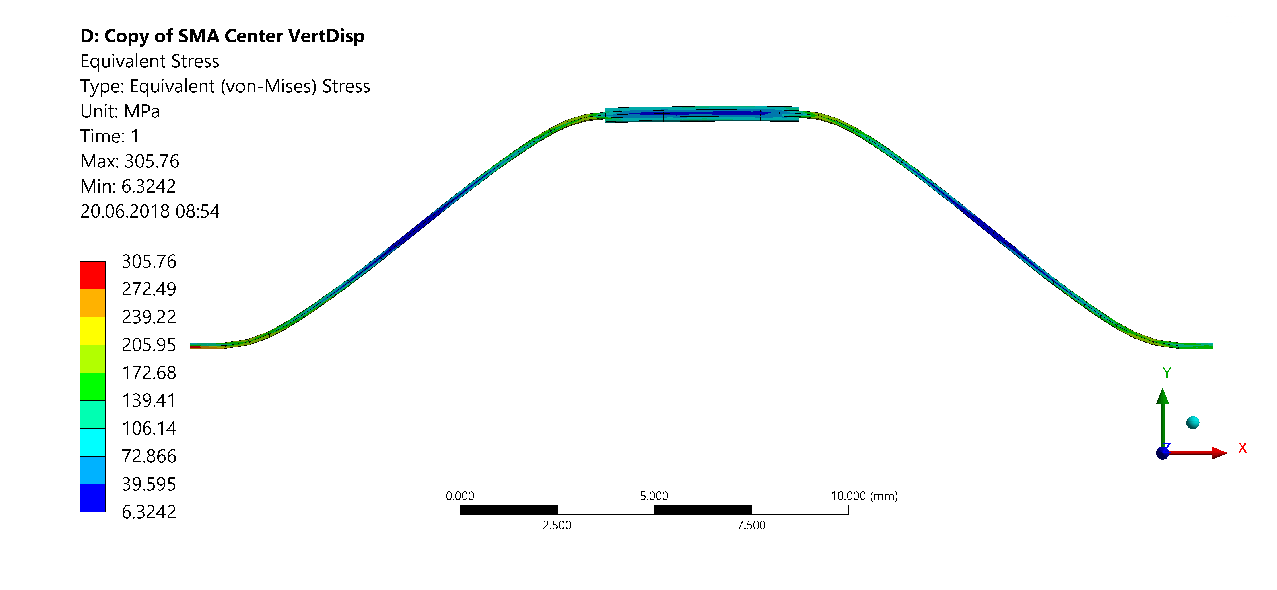
\includegraphics[width=\textwidth]{Figures/FigCentBumpBefore2x.eps}
			\caption{Before heating}
			\label{fig:modechangebefore}
    \end{subfigure}
		~
     %add desired spacing between images, e. g. ~, \quad, \qquad, \hfill etc.
      %(or a blank line to force the subfigure onto a new line)
    \begin{subfigure}[t]{0.45\textwidth}
			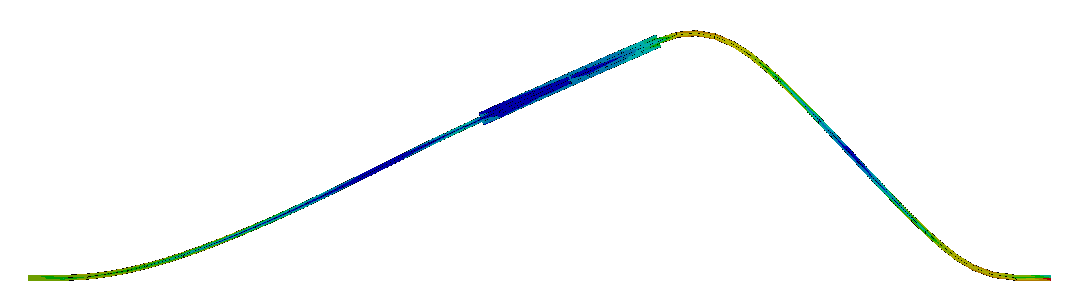
\includegraphics[width=\textwidth]{Figures/FigCentBumpAfter2x.eps}
			\caption{After heating}
			\label{fig:modechangeafter}
    \end{subfigure}
		\caption{Stable positions of the buckled beam}
		\label{fig:modechange}
\end{figure}

The direction in which the blade transitions is due to the convergence of the solution in the simulation. In an experimental scenario, the direction of the transformation can be controlled by creating an asymmetry in the thermal load or mechanical conditions. By applying a thermal load to either direction, the direction of the final stable mode can be chosen.\\

The creation of a buckled SMA system that can self activate would allow the possibility of creating compact micro-actuators that does not require external activation mechanisms. The goal of the study was to determine and pre-size the parameters that would enable an SMA buckled beam system to behave as a self-switching bistable actuator. This study also offers an overview of the advantages of using finite element modelling to simulate shape memory alloys and the shape memory effect. The work was able to successfully simulate the shape memory effect which corresponds closely to the behaviour of shape memory alloys as seen from experimental trials. The finite element modelling will be an effective tool to create complex actuators using such a material and its shape memory effect behaviour.

The simulations show that the optimization of the dimensions of the initial SMA blade alone cannot provide sufficient strain recovery to transition the buckled beam from one stable mode to another. This is due to the fact that the quantity of the material that transforms to the detwinned M phase due to the buckling is not sufficient to create enough vertical displacement so as to self-switch.

The work initially strived to vary arbitrary parameters so as to observe an effect on the vertical displacement and thus, subsequently the beams ability to self-actuate. The initial simulations conclude that the parameters that influence the self-switching are difficult to pinpoint. In figure \ref{fig:modechangeafter}, the stable mode after heating can be observed. The simulations show that by creating a blade with variable thickness, the behaviour of the system can be greatly affected. The thickened regions divide the beam into segments, allowing regions of the beam which are curved in the same direction to be actuated while regions that are curved in the opposite direction to not be actuated. This effect has been seen in \cite{rossiter_self-switching_2006} where the same principle is used for electrically stimulated self-switching buckled beams. The segmentation allows regions that will actuate in opposite directions to be reduced and thus further improve the vertical displacement.

\subsection{Test bench layout}
The test bench that was designed to measure the time response of the SMA actuator is constructed as shown in figure~\ref{fig:test_bench}.
\begin{figure}[H]
	\centering
	\def\svgwidth{0.5\columnwidth}
	\input{Figures/test_bench.pdf_tex}
	\caption{Layout of the test bench}
	\label{fig:test_bench}
\end{figure}

An SMA blade is fixed between two electrodes which allow an electrical current to flow through the system. In this setup, the right electrode is part of the main body of the test bench while the left electrode is placed on a linear guide in order for it to be able to move unidirectionally only. Using this mobile part, the blade is preconstrained while in its M phase i.e. at low temperature. A force sensor is then placed behind the left electrode and fixed to the bench to measure the force applied by the SMA actuator while it tries to return to its initial shape during the transition from the M phase to the A phase, i.e. heating.

\subsection{Thermal response enhancement}
SMA actuators are known for their high work output density but they are also known to be quite slow in terms of time response. The aim of this work is to optimize the heating of the SMA in critical sections and thus improve the force output and actuation times of the SMA actuator. The SMA blades are actuated using Joule heating where a current is passed through the blade and the internal resistance is used to heat the blade. Thus, the geometry of the blade is critical when optimizing the time response of the shape memory effect. The design of the SMA blades were created based on four factors as defined below and shown in figure \ref{fig:BladeSample} while also keeping the volume of material used constant:
\begin{enumerate}[label=\textbf{Factor $x_{\arabic*}$}:,align=left]
  \item Number of perforations along the width
  \item Position of the holes along the length
  \item Number of perforations along the length
  \item Orientation of the perforation
\end{enumerate}
The volume of material of the blade was also kept constant so as to have the same quantity of material to be heated during each run. This is controlled by ensuring that the thickness of blades are the same and that the total surface area is constant between each blade.

\begin{figure}[H]
	\centering
	\def\svgwidth{0.5\columnwidth}
	\input{Figures/SMA_LaserCut_revB.pdf_tex}
	\caption{Laser cut SMA blades based on the generated Hadamard matrix and the four factors.}
	\label{fig:BladeSample}
\end{figure}
The conventional option for the design of the test would be to design changes in the beam based on one factor at a time and observe the effect on the time response. This method is inefficient and time-consuming. Furthermore, the material is quite expensive, so extracting quality information for multiple construction factors from each blade is primordial. Thus a systematic design based on a Hadamard matrix that changes several variables simultaneously is performed. This allows to perform the analysis of the factor with respect to the time response in terms of the force-time derivative while reducing the number of runs and the quantity of material used.
\begin{figure}[H]
    \centering
    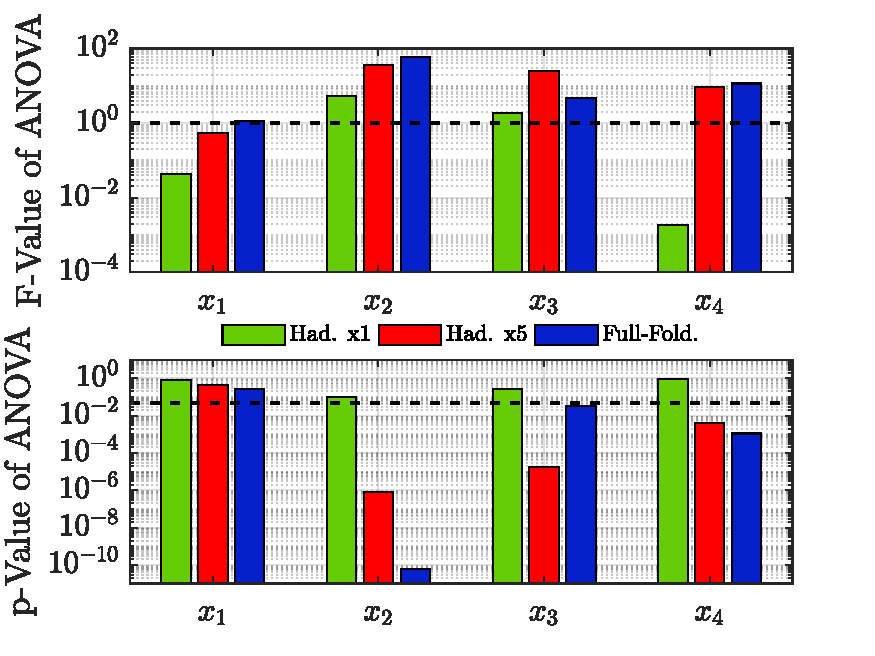
\includegraphics[width=0.53\textwidth]{Figures/fig_bar.pdf}
    \caption{Graph showing the influence of each factor with respect to the residual of the models and the corresponding confidence values.}
    \label{fig:bar1}
\end{figure}

A linear fit of the force derivative with respect to time $\frac{dF}{dt}$ was performed, in the form of $\frac{dF}{dt} \sim x_1+x_2+x_3+x_4 $ (in Wilkinson notation) for the Hadamard with one run, five runs, and the full fold-over. To check the significance of the SMA design parameters and their corresponding certainty, an Analysis of Variance (ANOVA) of this model is conducted.

The upper plot of figure \ref{fig:bar1} represents the ANOVA F-Value: the influence of each factor upon the experiment with respect to the residual of this model. It is desirable to obtain coefficients whose significance is high with F-value $\geq$ 1. The lower plot represents the ANOVA p-value, which is the probability of having validated a hypothesis by chance. In this case, the hypothesis is that factors have a non-zero influence in the model; meaning that small p-values (being sure that the parameters have a non-null influence) are desirable. As an arbitrary threshold, it was deemed that concluding results should have p-values $\leq$ 0.05 (marked in plot).

After the Had. x1, only $x_2$ and $x_3$ were slightly more significant than the residual of the model. Still, their p-values reflected a non-satisfactory certainty upon this affirmation, so it was decided to test the blades four additional times, leading to Had. x5. This time $x_2$ and $x_3$ became more influential, whereas $x_4$ newly became influential. Given their corresponding p-values, it could be affirmed that these three factors indeed affect the force vs time of SMAs; the longitudinal centring of the perforations, the number of them and their orientation, respectively.

Despite the Had. x5 approach, it was not clear if factor $x_1$ had small or no influence at all in the SMA performance. To gain further insight, and de-alias the results, eight new blades corresponding to the $-H$ experimental matrix were tested five times each, resulting in a full fold-over design. This analysis confirmed with high certainty the influence of factors $x_2$, $x_3$ and $x_4$. This time, however, it claimed a rather non-null influence of factor $x_1$, i.e. bigger than measurement noise. Nevertheless, the 0.28 p-value of factor $x_1$ indicates that the previous affirmation is inconclusive, and that this high influence might be product of randomness. This seems plausible given the very low F-values for factor $x_1$ and their evolution with the experimental procedures.

In conclusion, this work showed that the response of a SMA blade in terms of maximal force-time derivative can be optimized by carefully placed perforations. Indeed, an improvement by a factor of 3 could be observed between the highest and the lowest response in this experiment. Significant factors could be identified using a Hadamard matrix for the preparation of the samples and an ANOVA analysis of the results. The most relevant factor turned out to be the position of the perforations along the blade, followed by their longitudinal number and orientation.
